\documentclass{article}
\usepackage[utf8]{inputenc}
\usepackage{graphicx}

\begin{document}
\begin{center}
\huge Software Development Life-cycle Model
\end{center}
\section{Introduction}
We are working on large scale project. The time estimate of our project as estimated by COCOMO is around 8-10 months. Also, our client has asked us present us a working solution with some functionality, on the basis of which they will judge whether they want to continue working with us on this project. Also, taking in the fact that we have to present this solution as part of our SE project. We have decided to divide our project in multiple stages. These stages are divided on the basis of importance, implementation requirements and approximate time required for particular functionality at the end of all the stages we will have our final project which will be ready to deploy to large scale usage.
\section{Stages of Project}
\subsection{First Stage}
This is the first stage of our project and this is the stage we are aiming to present as the final submission of our Software Engineering Project. This stage will basically cover the implementation of bare bones of our project. If we are able to complete this stage quickly, we'll present the second stage of our project. The tasks we aim to achieve in this stage are:
\begin{enumerate}
\item Interface for Consumer
\item Interface for Pharmacy Seller
\item Interface for Administration 
\end{enumerate}
\subsection{Second Stage}
The second stage of our project will include several enhancements on the first stage. The result of this stage is what we will present as our first working solution to the client. This stage will include following things:
\begin{enumerate}
\item Nearest Pharmacy Location using Google Geo API
\item Integration of Medical Database with the inventory
\item Better UI and UX of the site.
\end{enumerate}
\subsection{Third Stage}
This stage includes all the developments we will do if clients decides to work further on this project with us. This stage includes basically includes all the ideas which the client wants in solution. Rather than being a stage in itself, it contains list of ideas and according to the ideas this stage may be will probably be divided into several stages. The ideas which we may implement in this stage are:
\begin{enumerate}
\item Automation of Prescription Verification
\item Making the solution platform compatible
\end{enumerate}
\section{SDLC Model Selection}
In our project each stage is incremental in terms of features and the final build holds all the features required by the customer. So as a result the Model which suits to our Software Development is the "Agile Model".
\subsection{Agile Model}
Agile SDLC model is a combination of iterative and incremental process models with focus on process adaptability and customer satisfaction by rapid delivery of working software product. Agile Methods break the product into small incremental builds. These builds are provided in iterations. Each iteration typically lasts from about one to three weeks. Every iteration involves cross functional teams working simultaneously on various areas like −
\begin{itemize}

\item    Planning
\item    Requirements Analysis
\item    Design
\item    Coding
\item    Unit Testing and
\item    Acceptance Testing

\end{itemize}

\begin{figure}
  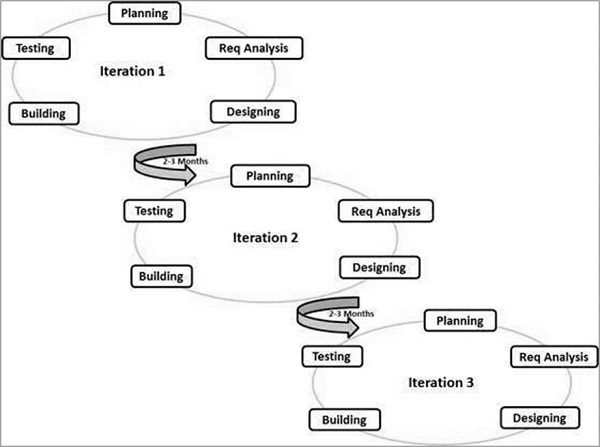
\includegraphics[width=\linewidth]{sdlc_agile_model}
\end{figure}

Following are the Agile Model Principles -

\begin{itemize}
\item   \textbf{Individuals and interactions} − In Agile development, self-organization and motivation are important, as are interactions like co-location and pair programming.

\item    \textbf{Working software} − Demo working software is considered the best means of communication with the customers to understand their requirements, instead of just depending on documentation.

\item    \textbf{Customer collaboration} − As the requirements cannot be gathered completely in the beginning of the project due to various factors, continuous customer interaction is very important to get proper product requirements.

\item    \textbf{Responding to change} − Agile Development is focused on quick responses to change and continuous development.
\end{itemize}

\subsection{Agile Model in our Software Development Process}
Each stage of our project can be modelled as an iteration of Agile Model. So in total we have at minimum 3 such iterations. Each iteration in our project may requires Planning, Requirement Analysis, Design, Coding and Testing. So depending upon the stage of our project we will have to choose a development model for each of our iterations. 
And for the first stage of our project we have decided to go with Waterfall Model. The reason for choosing Waterfall was good Requirement Analysis and some constraints of time.
\subsection{Waterfall Model} 
Waterfall approach was first SDLC Model to be used widely in Software Engineering to ensure success of the project. In "The Waterfall" approach, the whole process of software development is divided into separate phases. In this Waterfall model, typically, the outcome of one phase acts as the input for the next phase sequentially.
The sequential phases in Waterfall model are −
\begin{itemize}

\item    \textbf{Requirement Gathering and analysis} − All possible requirements of the system to be developed are captured in this phase and documented in a requirement specification document.

\item    \textbf{System Design} − The requirement specifications from first phase are studied in this phase and the system design is prepared. This system design helps in specifying hardware and system requirements and helps in defining the overall system architecture.

\item    \textbf{Implementation} − With inputs from the system design, the system is first developed in small programs called units, which are integrated in the next phase. Each unit is developed and tested for its functionality, which is referred to as Unit Testing.

\item    \textbf{Integration and Testing} − All the units developed in the implementation phase are integrated into a system after testing of each unit. Post integration the entire system is tested for any faults and failures.


\begin{figure}
  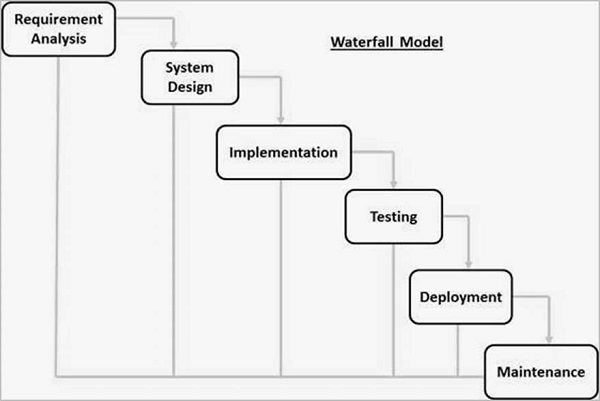
\includegraphics[width=\linewidth]{sdlc_waterfall_model}
\end{figure}

\end{itemize}
\end{document}

